\documentclass[aps,pra,reprint,superscriptaddress,longbibliography,nofootinbib,floatfix]{revtex4-2}
\usepackage[T1]{fontenc}
\usepackage{amsmath,amssymb,amsthm,bm,mathtools}
\usepackage{graphicx,booktabs,microtype}
\usepackage{tikz}
\usetikzlibrary{arrows.meta,positioning,calc,decorations.pathreplacing}
\usepackage[hidelinks]{hyperref}
\newcommand{\repolink}{\href{https://github.com/SamMausberg/returning-constructor}{\nolinkurl{github.com/SamMausberg/returning-constructor}}}
\usepackage[nameinlink,noabbrev]{cleveref}
\newtheorem{theorem}{Theorem}
\usepackage{aliascnt}
\newaliascnt{lemma}{theorem}
\newtheorem{lemma}[lemma]{Lemma}
\aliascntresetthe{lemma}
\newaliascnt{proposition}{theorem}
\newtheorem{proposition}[proposition]{Proposition}
\aliascntresetthe{proposition}
\newaliascnt{corollary}{theorem}
\newtheorem{corollary}[corollary]{Corollary}
\aliascntresetthe{corollary}
\crefname{lemma}{Lemma}{Lemmas}
\Crefname{lemma}{Lemma}{Lemmas}
\crefname{proposition}{Proposition}{Propositions}
\Crefname{proposition}{Proposition}{Propositions}
\crefname{corollary}{Corollary}{Corollaries}
\Crefname{corollary}{Corollary}{Corollaries}
% APS style capitalizes numbered references mid-sentence.
\crefname{theorem}{Theorem}{Theorems}
\crefname{table}{Table}{Tables}
\theoremstyle{definition}\newtheorem{definition}[theorem]{Definition}
\newcommand{\Tr}{\operatorname{Tr}}
\newcommand{\id}{\operatorname{id}}
\newcommand{\rank}{\operatorname{rank}}
\newcommand{\supp}{\operatorname{supp}}
\newcommand{\norm}[1]{\left\lVert#1\right\rVert}
\newcommand{\ket}[1]{|#1\rangle}
\newcommand{\bra}[1]{\langle#1|}
\newcommand{\SW}{\mathsf S}
\newcommand{\ha}{h_2}
\newcommand{\Pone}{\mathcal P_1}
\newcommand{\positive}[1]{\left[#1\right]_+}
\DeclareMathOperator{\Bin}{Bin}
\setlength{\emergencystretch}{1em}
\newcommand{\statement}[1]{\input{statements/#1.tex}}

\usepackage{capt-of}
\hypersetup{pdftitle={Memory return in quantum machines},pdfauthor={Samuel Mausberg},pdfsubject={Closed quantum memories and repeated homogenization}}
% Natural spacing at column ends instead of stretched display and float gaps.
\raggedbottom
\begin{document}
\title{Memory return in quantum machines}
\author{Samuel Mausberg}
\affiliation{Independent researcher}
\email{samuelmausberg@gmail.com}
\date{October 2, 2026}
\begin{abstract}
We ask whether a quantum machine can repeatedly transform fresh inputs while returning its memory to its initial state. We obtain three results. First, exact memory return prevents a closed machine from purifying maximally mixed inputs, for every initial memory state. With return tolerance $\delta$, exact purification of $n$ qubits requires $n/\delta+O(n)$ memory qubits; independent randomization requires only $\lceil n/2\rceil$ and allows exact return. Second, one use of the coherent quantum homogenizer requires a reservoir of size $\Theta(\log^2(1/\epsilon)/\delta^2)$ for output error $\epsilon$ and return error $\delta$. Accurate repeated output marginals can coexist with small return error, but two-output correlations impose $\epsilon+\delta/2\ge1/4$ when independent outputs and return after every use are required. Third, the exact repeated dynamics give identical iterated deterioration limits in both directions, while a forward-capable product initializer makes the published first-use capability infimum tend to zero. These results separate the return of a memory's reduced state from its ability to supply fresh independent randomness.
\end{abstract}
\maketitle

\section{Introduction}

Can a machine repeatedly change the state of a quantum system and still return to its starting condition? The answer depends on what we ask the machine to preserve. A memory may recover its reduced state while becoming correlated with the systems it has released. Such correlations matter as soon as we try to use those systems together.

Consider a machine holding one fair classical bit. Each incoming bit is zero. The machine copies its stored bit onto the input and releases the result, leaving its memory unchanged. Every output is fair, however many inputs arrive. Yet the entire output string is either all zeros or all ones. After seeing the first output, we can predict all the others. This repeatable randomizer, a special case of the random-unitary memory channels studied by Ryb\'{a}r and Ziman~\cite{rybar}, will serve as our running example.

For a user who tests one output at a time, the machine works indefinitely. A user who needs independent random bits receives a different resource. We therefore distinguish accuracy of each output marginal from accuracy of the joint output state. We also require the memory to return after each use, so that it can be inspected whenever another input is about to arrive. These choices allow us to ask quantitatively how much memory repeated transformation consumes.

The reverse transformation brings entropy into the question. A machine that changes fresh fair bits into zeros must retain the entropy removed from them. We show that exact return of its memory prevents this for every initializer. Approximate return behaves differently as memory dimension grows: an increasingly large mixed register can absorb entropy while moving only a small trace distance. We give a fixed-unitary construction that controls this movement after every use and compare it with a spectral lower bound.

We then examine the coherent quantum homogenizer, in which each input undergoes partial swaps with a reservoir. This circuit underlies the proposal of constructor-based irreversibility in Ref.~\cite{prl}. Its finite memory makes it possible to study the physical cost of returning a machine without replacing its internal correlations by a product state. We find a small-return asymmetry for output marginals, derive a sharp one-use reservoir cost, and identify a two-output obstruction to independent service. The exact dynamics also let us compare the deterioration criteria used in the original Letter and later treatments. We give that comparison in Appendixes~\ref{app:relaxation}, \ref{app:capable}, and~\ref{app:audit}.

\section{States, outputs, and memory return}\label{sec:contracts}

We write $p=\ket0\bra0$ and $\tau=I/2$. The forward transformation is $p\to\tau$, and the reverse is $\tau\to p$. A closed device has a memory $R$ of dimension $D=2^m$ in an initial state $\sigma_0$ independent of the inputs. At every visit, it applies the same unitary to the incoming qubit and $R$, then releases that qubit. The memory count $m$ includes clocks, buffers, retained random seeds, and workspace. We allow mixed initial memory and keep track of that resource. No register is reset or discarded during operation.

Let $\Omega_n$ be the first $n$ outputs jointly, $\rho_j$ the $j$th output, and $\sigma_j$ the memory after that visit. We use trace distance and squared Uhlmann fidelity,
\begin{align}
 T(\rho,\sigma)&=\tfrac12\norm{\rho-\sigma}_1,\nonumber\\
 F(\rho,\sigma)&=\left(\Tr\sqrt{\sqrt\rho\,\sigma\sqrt\rho}\right)^2.
 \label{eq:conventions}
\end{align}
Entropies and the binary entropy $\ha$ are measured in bits; $\ln$ denotes the natural logarithm.

For target state $b$, \emph{marginal service} means
\begin{equation}
 \max_{1\le j\le n}T(\rho_j,b)\le\epsilon,
 \label{eq:marginal}
\end{equation}
and \emph{joint service} means
\begin{equation}
 T(\Omega_n,b^{\otimes n})\le\epsilon.
 \label{eq:joint}
\end{equation}
The latter includes independence and controls every shorter output block by partial trace. Marginal accuracy refers to unconditional output states.

Our return requirement is
\begin{equation}
 \max_{1\le j\le n}T(\sigma_j,\sigma_0)\le\delta.
 \label{eq:return}
\end{equation}
We call this \emph{prefix return}. Endpoint return checks only the memory after visit $n$. Correlations with released outputs are retained throughout the dynamics, while Eq.~\eqref{eq:return} tests the memory's reduced state. We write $m_-^{\mathrm{ret}}(n,0,\delta)$ for the least number of memory qubits that give $n$ exact pure outputs from maximally mixed inputs with prefix return tolerance $\delta$; joint or marginal superscripts distinguish the corresponding approximate-output costs.

The fair-bit machine illustrates these definitions directly:
\begin{equation}
 \rho_j=\tau,\qquad \sigma_j=\tau,\qquad
 \Omega_n=\frac{\ket{0^n}\bra{0^n}+\ket{1^n}\bra{1^n}}2.
 \label{eq:fairbit}
\end{equation}
Its marginal accuracy and return error vanish. Its outputs share the same random bit, as shown in Fig.~\ref{fig:fairbit}.

\begin{table}[t]
\caption{Notation for a closed device and for its homogenizer specialization. All errors are trace distances unless fidelity is written.}
\label{tab:notation}
\begin{ruledtabular}
\begin{tabular}{lp{.68\columnwidth}}
$n$ & Number of inputs served\\
$m=\log_2D$ & Accessible memory, in qubits\\
$M$ & Number of homogenizer reservoir cells\\
$\epsilon,\delta$ & Output error and memory-return tolerance\\
$\rho_j,\Omega_n$ & Output $j$ and the first $n$ outputs jointly\\
$\sigma_j$ & Memory state after input $j$\\
$u=\sin^2\eta$ & Partial-swap strength; $q=1-u$\\
\end{tabular}
\end{ruledtabular}
\end{table}

\begin{figure}[!t]
\centering
\begin{tikzpicture}[x=1cm,y=1cm,>=Latex,font=\footnotesize,line width=.6pt]
\draw[fill=black!7,draw=none] (.62,.22) rectangle (7.4,-.22);
\foreach \y/\label in {0/{R:\tau},-.6/{S_1:p},-1.2/{S_2:p},-1.8/{S_3:p}}{
 \draw (.7,\y)--(7.3,\y);
 \node[anchor=east] at (.55,\y) {$\label$};
 \node[anchor=west] at (7.4,\y) {$\tau$};
}
\foreach \x/\y in {2/-.6,4/-1.2,6/-1.8}{
 \fill (\x,0) circle(1.8pt);
 \draw (\x,0)--(\x,\y);
 \draw[fill=white] (\x,\y) circle(.10);
 \draw (\x-.1,\y)--(\x+.1,\y);
 \draw (\x,\y-.1)--(\x,\y+.1);
}
\node at (4,-2.34) {Outputs: $000$ or $111$, each with probability $1/2$};
\end{tikzpicture}

\caption{A fair-bit randomizer. The upper wire is a memory qubit initially in $\tau=I/2$. At each visit it controls a CNOT onto a fresh qubit in $p=\ket0\bra0$. The memory remains in $\tau$ and every released qubit has state $\tau$. Measuring all outputs in the computational basis gives only the strings $0^n$ and $1^n$, each with probability $1/2$. Thus exact return of the memory and exact single-output accuracy coexist with perfect correlations between outputs.}
\label{fig:fairbit}
\end{figure}

\section{Memory return in a closed device}\label{sec:general}

\subsection{The entropy balance}

When the incoming qubits are maximally mixed, the entropy absent from the outputs must appear in the memory. Correlations tighten that balance. The following statement also keeps the dependence on memory dimension visible.

\statement{thm_entropy}

Every bit of entropy removed from the outputs must increase the memory entropy. Correlations between the outputs and memory use additional capacity. Unitary invariance of entropy, subadditivity, and Audenaert's continuity bound~\cite{audenaert} turn this balance into the inequalities above; Appendix~\ref{app:general} gives the proof.

Exact return has a particularly simple consequence.

\statement{cor_exactreturn}

With its entropy restored, the memory has no capacity left to absorb entropy from the inputs. The outputs must retain their entire initial entropy, and the equality case also removes their correlations with the memory. The proof is in Appendix~\ref{app:general}.

We can express the approximate-return cost through the entropy defect
\begin{equation}
 \mathfrak r(D,\delta)=\ha(\delta)+\delta\log_2(D-1).
 \label{eq:defect}
\end{equation}
If this defect is $o(n)$, output error tending to zero is incompatible with reverse service. For fixed finite memory, the defect remains bounded as more inputs arrive. When the memory grows, the factor $\log_2D$ measures its capacity to absorb entropy despite a small trace change.

An initially pure memory obeys the additional bound
\begin{equation}
 F(\sigma_n,\sigma_0)\le2^{-n}+e_{\rm all},\qquad
 e_{\rm all}=1-\bra{0^n}\Omega_n\ket{0^n}.
 \label{eq:pure-return}
\end{equation}
Here $e_{\rm all}\le\epsilon$ under joint accuracy and $e_{\rm all}\le n\epsilon$ under marginal accuracy. The initial global state has largest eigenvalue $2^{-n}$. This bounds the probability that both the outputs and the memory occupy their prescribed pure states.

At one use, Eq.~\eqref{eq:pure-return} requires $\delta\ge1/2-\epsilon$. This will be the reverse obstruction for the homogenizer.

\subsection{Randomization with exact return}

The fair-bit machine supplies the least demanding form of forward service. Independent outputs require a larger memory, but they can still leave its reduced state unchanged.

\statement{thm_forwardoptimal}

A mixed memory can distribute two independent Pauli labels per qubit among the released outputs while preserving its own reduced state. The output rank makes this capacity precise: pure inputs and a memory of initial rank $r_0$ give an output state of rank at most $Dr_0\le D^2$.

To attain that rank, we initialize the memory in $\tau^{\otimes m}$ and, at each visit, apply a Hadamard to the input, a CNOT from the input to the leading memory qubit, a Hadamard to that memory qubit, and a cyclic memory rotation. The first two visits to each cell encode two independent Pauli labels. Their trace orthogonality gives the stated output error, while the memory's mixture of unitary conjugations preserves $\tau^{\otimes m}$.

This factor-of-two saving is the catalytic-randomness mechanism of Boes and collaborators~\cite{boes}, with its correlational resource analyzed by Lie and Jeong~\cite{lie}. Counted Pauli streaming also appears in Ref.~\cite{douglas}. The cyclic implementation used here needs no additional clock for the prescribed pure input. Appendix~\ref{app:general} gives its full construction and covers every horizon, including $n>2m$.

\subsection{Purification with approximate return}

To understand how closely the reverse machine can return, we allow a mixed initializer whose spectrum extends over many scales. Approximate catalytic erasure with increasing dimension was established by Ng and collaborators~\cite{ng}. Here we control the memory after every intermediate visit using one fixed cyclic unitary.

\statement{thm_dyadic}

The construction places zero bits at the head of a register with a dyadic probability distribution. A visit emits the leading zero and appends the incoming fair bit. Most of the spectrum is unchanged by this dilation; the probability mass that moves after $t$ visits is exactly $t/(m-n+2)$. Figure~\ref{fig:shift} shows the register, and Appendix~\ref{app:general} gives the initializer and the probability calculation.

\begin{figure}[!t]
\centering
\begin{tikzpicture}[x=1cm,y=1cm,>=Latex,font=\footnotesize,line width=.6pt]
\node[anchor=east] at (.52,0) {$\sigma_0$};
\draw[fill=white] (.7,-.30) rectangle (2.4,.30);
\draw[fill=black!7] (2.4,-.30) rectangle (7.4,.30);
\node at (1.55,0) {$0^n$};
\node at (4.9,0) {dyadic tail};
\draw[->] (4.05,-.5)--(4.05,-1.1);
\node[anchor=west] at (4.2,-.8) {$t$ cyclic swaps};
\node[anchor=east] at (.52,-1.6) {$\sigma_t$};
\draw[fill=white] (.7,-1.9) rectangle (2.2,-1.3);
\draw[fill=black!7] (2.2,-1.9) rectangle (5.8,-1.3);
\draw[fill=black!17] (5.8,-1.9) rectangle (7.4,-1.3);
\node at (1.45,-1.6) {$0^{n-t}$};
\node at (4,-1.6) {dyadic tail};
\node at (6.6,-1.6) {$\tau^{\otimes t}$};
\node at (4.05,-2.35) {$t$ pure outputs released; $m$ memory qubits retained};
\end{tikzpicture}

\caption{A closed register that purifies $n$ fresh maximally mixed qubits. The $m$-qubit initializer contains $n$ leading zeros and a diagonal tail with the dyadic spectrum in Eq.~\eqref{eq:dyadicspectrum}. Each use swaps out the leading bit and moves the incoming fair bit to the tail. After $t\le n$ uses, the released qubits are exactly $p^{\otimes t}$ and the memory has gained $t$ bits of entropy. Its trace distance from the initializer is $t/(m-n+2)$ for $m\ge2n$. Every register shown is retained and counted.}
\label{fig:shift}
\end{figure}

A spectral converse narrows the additive gap left by the entropy inequality. It is the closed-unitary form of the endpoint catalyst bound in Ref.~\cite{ng}.

\statement{prop_spectralreturn}

Pure outputs separate from everything retained in the device. The memory therefore carries the full incoming mixture, which appears in its spectrum as repeated, diluted copies of the initial eigenvalues. Summing the trace-distance constraints across successive groups of eigenvalues gives Eq.~\eqref{eq:spectralreturn}; Appendix~\ref{app:general} supplies the argument.

A return tolerance therefore measures a resource cost even for a device that appears almost unchanged. Exact purification requires $n/\delta+O(n)$ memory qubits as $\delta$ decreases, whereas exact independent randomization uses $n/2+O(1)$ and returns its memory exactly. The fair-bit version of forward service uses one qubit for every horizon. Figure~\ref{fig:costs} shows the finite-size bounds for independent outputs.

\begin{figure*}[!t]
\centering
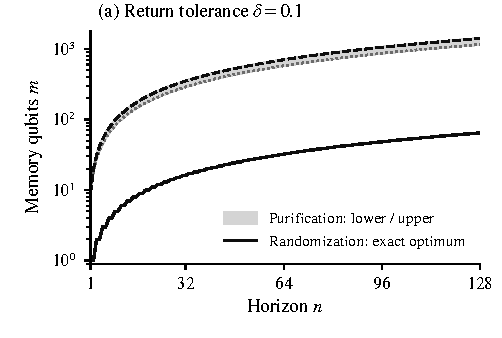
\includegraphics[width=.48\textwidth]{figures/cost_horizon.pdf}\hfill
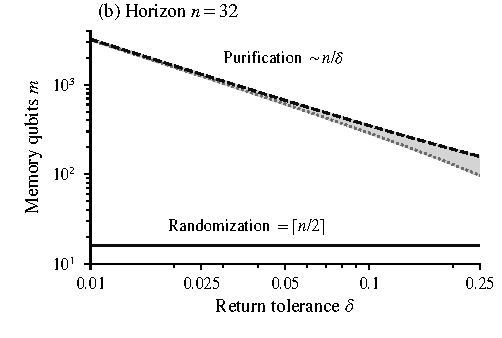
\includegraphics[width=.48\textwidth]{figures/cost_tolerance.pdf}
\caption{Memory needed to convert pure qubits to independent maximally mixed outputs, or to reverse that transformation, in a closed device allowing mixed initialization and return after every use. (a) Horizon $n$ at fixed return tolerance $\delta=0.1$. (b) Return tolerance at $n=32$. The solid curve is the exact randomization optimum $\lceil n/2\rceil$, attained with zero return error. For purification, the shaded region lies between the spectral lower bound~\eqref{eq:spectralmemory} and the achievable dyadic upper bound~\eqref{eq:erasurecost}; its edges are dotted and dashed, respectively. All values are exact integer evaluations, including rounding. The region brackets the optimum rather than identifying a finite-size cost.}
\label{fig:costs}
\end{figure*}

For approximate outputs, we retain a classical flag as part of the memory. With probability $w$ the flag selects the purification device; otherwise the device leaves the input and memory unchanged.

We take $w=1-\epsilon$ for joint service and $w=1-2\epsilon$ for marginal service. Counting the flag gives
\begin{equation}
 m\le1+\max\left\{2n,\left\lceil\frac{wn}{\delta}\right\rceil+n-2\right\}.
 \label{eq:flagupper}
\end{equation}
Together with Theorem~\ref{thm:entropy}, this yields, for fixed $0\le\epsilon<1/2$,
\begin{equation}
 \lim_{\delta\downarrow0}\limsup_{n\to\infty}
 \frac{\delta\,m_-^{\mathrm{ret,joint}}(n,\epsilon,\delta)}n
 =1-\epsilon.
 \label{eq:jointapproxrate}
\end{equation}
The corresponding marginal coefficient lies between $1-\ha(\epsilon)$ and $1-2\epsilon$.

\section{The repeated quantum homogenizer}\label{sec:homogenizer}

The coherent homogenizer replaces the freely chosen memory unitary by a sequence of partial swaps. Its reservoir consists of $M$ qubits in $b^{\otimes M}$. Each independent input in state $a$ visits the cells in the same order through
\begin{equation}
 U_\eta=\cos\eta\,I+i\sin\eta\,\SW,
 \qquad 0<\eta\le\pi/2.
 \label{eq:partialswap}
\end{equation}
We write $u=\sin^2\eta$ and $q=1-u$. The forward initializer is $\tau^{\otimes M}$, the reverse initializer $p^{\otimes M}$. This is the partial-swap machine introduced by Ziman, Bu\v{z}ek, and collaborators~\cite{ziman}, closely related to the thermalizing machines of Ref.~\cite{scarani}.

Let $\Phi_{b,k}$ be the channel that introduces one fresh qubit in state $b$, sweeps it through a $k$-qubit block, and traces it out. The repeated circuit has two exact evaluations:
\begin{align}
 \Omega_{M,n}&=\Phi_{b,n}^{\,M}(a^{\otimes n}),\nonumber\\
 \sigma_{M,n}&=\Phi_{a,M}^{\,n}(b^{\otimes M}).
 \label{eq:column}
\end{align}
Changing from rows to columns exchanges only gates on disjoint wires. This collision-model rearrangement appears in Refs.~\cite{gp,cascade}. Figure~\ref{fig:grid} shows the two orders. It lets us keep all correlations while working with whichever block is smaller.

\begin{figure}[!t]
\centering
\begin{tikzpicture}[x=.72cm,y=.72cm,font=\footnotesize,line width=.6pt]
\foreach \offset/\head in {0/{Row order},6/{Column order}}{
 \node at (\offset+2,1.15) {\head};
 \foreach \j in {1,2,3}{\node at (\offset+\j,.48) {$R_{\j}$};}
 \foreach \i in {1,2,3}{
  \node[anchor=east] at (\offset+.42,-\i+.35) {$S_{\i}$};
  \foreach \j in {1,2,3}{
   \draw[fill=black!7] (\offset+\j-.34,-\i+.01) rectangle (\offset+\j+.34,-\i+.69);
   \ifnum\offset=0
    \pgfmathtruncatemacro{\num}{3*(\i-1)+\j}
   \else
    \pgfmathtruncatemacro{\num}{3*(\j-1)+\i}
   \fi
   \node at (\offset+\j,-\i+.35) {\num};
  }
 }
}
\node at (4.85,-1.65) {$=$};
\end{tikzpicture}

\caption{Two evaluations of a repeated partial-swap circuit. Rows label successive inputs $S_i$, and columns label reservoir cells $R_j$. Each square acts on the two wires named by its row and column; the number gives its position in the evaluation order. Changing from row order to column order reverses only pairs on distinct rows and columns, whose gates commute. The total unitary is unchanged. Tracing a completed column gives a fresh-ancilla channel on the output block, yielding Eq.~\eqref{eq:column}.}
\label{fig:grid}
\end{figure}

\subsection{Return after one use}

A weak partial swap transfers little information to each reservoir cell, but the accumulated disturbance depends on the whole reservoir. Its purity gives an exact measure of that accumulation. A fourth-moment bound then converts purity into a trace-distance lower bound.

\statement{thm_moments}

The squared disturbance accumulates by an amount of order $u^2$ per fresh cell. A large reservoir can therefore contain many individually small changes whose combined size remains measurable.

To obtain the identity, we evolve the initial input Pauli operator and separate its coefficient on the system identity. Adding a fresh cell changes the normalized second moment by $a\mapsto a+u^2(1-a)$. The fourth moment bounds how strongly the spectral weight can concentrate. Interpolation between the first, second, and fourth moments gives Eq.~\eqref{eq:returnlower}. The derivation is in Appendix~\ref{app:moments}.

\statement{cor_singlecost}

The first output has trace error exactly $q^M/2$. Accuracy thus needs a total coupling of order $Mu\sim\ln(1/\epsilon)$, while return requires $u\sqrt M$ to remain of order $\delta$. Combining these two scales gives the logarithm-squared reservoir cost. Appendix~\ref{app:moments} retains the constants and integer rounding.

For a prescribed coupling, increasing the reservoir size eventually conflicts with return. With $\ell=\ln[1/(2\epsilon)]$ and $0<\epsilon,\delta\le1/4$, necessary conditions are
\begin{equation}
 \frac{\ell}{-\ln(1-u)}\le M\le\frac{128\delta^2}{u^2}.
 \label{eq:prescribed1necess}
\end{equation}
The inequalities $\ell/u\le M\le4\delta^2/u^2$ are sufficient, with integer rounding. At weak coupling these intervals match up to constants: feasibility requires $u\ell$ of order at most $\delta^2$.

The reverse initializer is pure, so Eq.~\eqref{eq:pure-return} applies. In fact, its one-use tradeoff is exact:
\begin{equation}
 T(\rho_{M,1},p)=\frac{q^M}{2},\qquad
 T(\sigma_{M,1},p^{\otimes M})=\frac{1-q^M}{2}.
 \label{eq:reverse-first}
\end{equation}
Accurate purification and small return error already conflict at the first input.

\subsection{Repeated marginal service}

Repeated forward service must supply excitations from the reservoir to the initially zero inputs. Because the reservoir starts maximally mixed, its initial excitation number is binomially distributed. Returning that distribution close to its starting point limits the transport it can support.

\statement{thm_transport}

Every randomized output draws excitations from the reservoir. Returning the reservoir requires this transport to fit within the width of its initial number distribution.

We prove this by coupling the initial excitation number $K$ to the final output and reservoir counts $X,Y$. Conservation gives $K=X+Y$ and $0\le X\le n$. Trace distance bounds the shift of each number threshold, and a binomial tail estimate bounds how many thresholds contribute appreciably. The argument uses endpoint return alone; Appendix~\ref{app:transport} gives the details.

For an upper bound, let $\Phi$ be the one-row reservoir channel. Contractivity gives $T(\Phi^j(\sigma_0),\sigma_0)\le jT(\Phi(\sigma_0),\sigma_0)$. We obtain
\begin{align}
 \max_{j\le n}T(\sigma_{M,j},\tau^{\otimes M})
 &\le\tfrac n2u\sqrt M,\label{eq:telescope}\\
 \max_{j\le n}T(\rho_{M,j},\tau)
 &\le\tfrac12q^M+\tfrac{n-1}{2}u\sqrt M.
 \label{eq:legacyupper}
\end{align}
A second estimate uses the rotational symmetry of the fresh-$\tau$ column channel to control output accuracy independently of the return telescope.

\statement{lem_collective}

Weak collisions wash out each spin's polarization while allowing correlations between spins to persist. The channel's second-order generator is collective depolarization. Every one-qubit Pauli observable belongs to its rank-one tensor sector, on which the generator has eigenvalue $-1$. A uniform bound on the exact channel's Taylor remainder controls the finite step size. We give that estimate in Appendix~\ref{app:collective}.

\statement{thm_manyupper}

Both designs spread the disturbance across many weak collisions. The first controls output accuracy through the changing reservoir state; the second uses the decay of one-qubit observables.

For the first design, the terms in Eq.~\eqref{eq:legacyupper} divide the allowed output error between first-use accuracy and accumulated memory change. For the second, Lemma~\ref{lem:collective} controls the outputs while Eq.~\eqref{eq:telescope} controls return. The proof and the parameter checks appear in Appendix~\ref{app:transport}.

At prescribed weak coupling, a sufficient interval is
\begin{equation}
 \frac{2L}{\eta^2}\le M\le\frac{4\delta^2}{n^2\sin^4\eta},
 \qquad \eta\le\frac{3}{8n^3}.
 \label{eq:prescribedmany}
\end{equation}
The first-use interval and excitation-transport lower bound continue to apply. Finite-horizon resource questions and individual-cell disturbance also appear in Refs.~\cite{vm,beever}; the return distances here refer to the whole correlated reservoir.

\subsection{What two outputs reveal}

The fair-bit randomizer warns that accurate marginals can conceal correlations. In the homogenizer, a singlet measurement on the first two outputs detects the same issue quantitatively.

\statement{thm_singlet}

Two independent fair qubits occupy the singlet with probability $1/4$. Keeping the reservoir close to its initial state limits how quickly that population can build up in the outputs.

The adjoint two-cell channel sends the singlet projector to $u^2I/4+(1-u^2)P_-$. Iteration determines the singlet population. The independent target $\tau^{\otimes2}$ has singlet probability $1/4$, and the one-use purity identity ties the deficit to the first return error. Appendix~\ref{app:singlet} gives the calculation.

At fixed $n$, this correlated behavior has a simple weak-coupling limit. For $\eta=M^{-\alpha}$ with $1/3<\alpha<1/2$, the reservoir returns in trace distance and
\begin{equation}
 \Omega_{M,n}\longrightarrow\frac{\Pi_{\mathrm{sym}}}{n+1},
 \label{eq:collectivetwirl}
\end{equation}
where $\Pi_{\mathrm{sym}}$ projects onto the symmetric $n$-qubit subspace. Each output is maximally mixed, while the joint trace distance from $\tau^{\otimes n}$ tends to $1-(n+1)/2^n$. At two outputs the distance is $1/4$. This is the collective counterpart of the fair-bit example: the returned memory accompanies a correlated family of individually correct outputs. Figure~\ref{fig:singletdata} resolves both errors along a weak-coupling sequence.

\begin{figure}[!t]
\centering
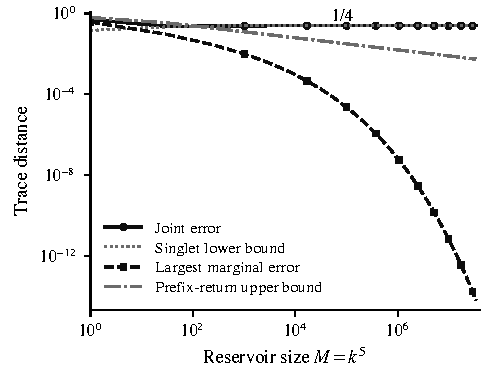
\includegraphics[width=\columnwidth]{figures/singlet_data.pdf}
\caption{Two-input randomization $p^{\otimes2}\to\tau^{\otimes2}$, where $p=\ket0\bra0$ and $\tau=I/2$. The reservoir starts in $\tau^{\otimes M}$, with $M=k^5$, $\eta=2\arctan[1/(2k^2)]$, $k=1,\ldots,32$. The largest marginal trace error falls while the joint error approaches $1/4$. The dotted curve is the singlet lower bound $(1-u^2)^M/4$; the dash-dotted curve bounds prefix return by $\min\{1,u\sqrt M\}$. Exact rational channel entries, 512-bit outward-rounded matrix powers, and enclosed spectral radicals give trace-error intervals narrower than $5\times10^{-114}$. Code and rational interval endpoints accompany the figure.}
\label{fig:singletdata}
\end{figure}

\section{Retaining the ability to act again}\label{sec:ability}

Constructor theory describes a constructor by its continued ability to perform a task. Deutsch allows its other attributes to change after use~\cite{deutsch}. The information paper represents attributes by sets of states~\cite{information}, and the thermodynamics paper allows microscopic changes within a constructor attribute~\cite{thermo}. The Letter similarly describes remaining within a suitable set of states~\cite{prl}. Together, these formulations direct attention to the transformations the machine can still perform.

For prescribed independent inputs and unconditional marginal accuracy, an invariant capability set captures that requirement. Let $\Phi_a$ update the memory and $\mathcal O_a$ produce the current output. Define
\begin{align}
 V_\epsilon&=\{\sigma:T(\mathcal O_a(\sigma),b)\le\epsilon\},\nonumber\\
 C_\epsilon&=\bigcap_{j\ge0}\Phi_a^{-j}(V_\epsilon).
 \label{eq:capabilityinvariant}
\end{align}
The inverse notation means set preimage. Membership in $C_\epsilon$ means that every horizon is served at tolerance $\epsilon$, and $\Phi_a(C_\epsilon)\subseteq C_\epsilon$. This is the fixed-error version of the nested capability sets in Refs.~\cite{vm,thesis}.

Memory return provides a useful sufficient comparison for a fixed future experiment supplied independently of earlier outputs: trace distance bounds the change of every outcome probability. Continued ability can also survive a large state change, as when a clock advances to an orthogonal state. The fair-bit machine illustrates the other direction. Its unconditional memory state returns exactly, but observing one output determines the next. Asking for independent outputs therefore changes the operational requirement.

The deterioration ratios introduce further choices. The published first-use numerator differs from the later current-output numerator, and their limiting procedures differ as well. The exact current-error ratio has opposite iterated limits in both task directions; Fig.~\ref{fig:ratios} shows finite-size slices. A first-use-capable product initializer also makes the Letter's capability infimum tend to zero. We give the proofs in Appendixes~\ref{app:relaxation} and~\ref{app:capable}, with the version-specific definitions in Appendix~\ref{app:audit}.

A final distinction concerns the horizon. Serving each finite horizon with a sufficiently large device has quantifiers $\forall n\,\forall\epsilon>0\,\exists D<\infty$. Unlimited reuse instead places the finite device before the universal horizon. The fair-bit machine meets that uniform marginal requirement. For independent joint outputs, every fixed finite memory has error tending to one when the input and target entropy densities differ; Appendix~\ref{app:finite} proves this statement.

\begin{figure*}[!t]
\centering
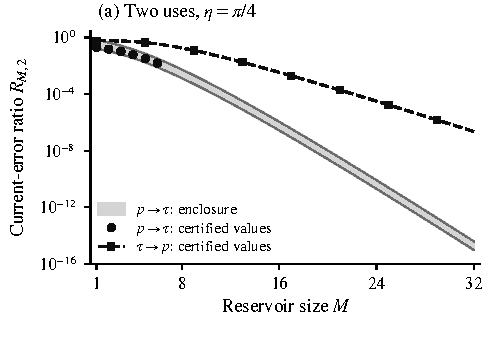
\includegraphics[width=.48\textwidth]{figures/ratio_reservoir.pdf}\hfill
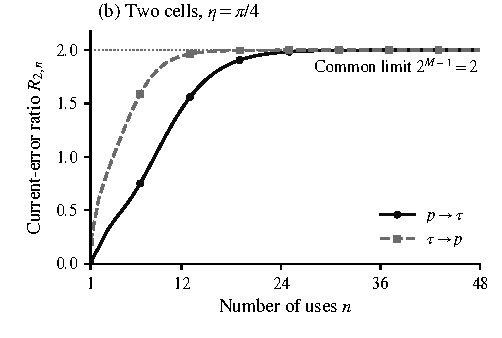
\includegraphics[width=.48\textwidth]{figures/ratio_uses.pdf}
\caption{The current-output infidelity divided by reservoir return fidelity, $R_{M,n}$ of Eq.~\eqref{eq:ratiodef}, for $p=\ket0\bra0$ and $\tau=I/2$ at $\eta=\pi/4$. (a) At two uses, both directions tend to zero as the reservoir grows. The gray forward band is the rigorous enclosure $e_{M,2}\le R_{M,2}\le4e_{M,2}$, where $e_{M,2}=1-F(\rho_{M,2},\tau)$ is rigorously enclosed from the exact two-cell channel. Forward markers at $M\le6$ use exact reservoir matrices with certified spectral root isolation; the reverse curve uses an exact conditional two-cell channel for its denominator. (b) With two reservoir cells, both ratios tend to $2^{M-1}=2$. Both curves use exact rational memory updates and enclosed square roots. Certified-value interval widths are below $10^{-28}$. Lines join integer samples. These slices display the common limits, although the finite-size ratios differ.}
\label{fig:ratios}
\end{figure*}

\section{Resource comparison}\label{sec:resources}

Table~\ref{tab:return} gathers the results with return after every use. The two freely chosen-memory constructions establish the general asymmetry: independent randomization can return the memory exactly, while exact purification has a memory cost proportional to the horizon divided by the allowed return error. The homogenizer has a sharper restriction because its initializer and excitation-conserving gate are fixed. Its small-return forward operation survives for marginal outputs, and the first two outputs already distinguish it from independent service.

\begin{table*}[t]
\caption{Memory requirements with whole-memory return after every use. The unrestricted-device rows allow arbitrary mixed initialization and count all accessible memory. The homogenizer keeps its designated product initializer and uses trace-distance output error $\epsilon$. The stated small-error ranges and constants are given in the referenced equations.}
\label{tab:return}
\begin{ruledtabular}
\begin{tabular}{p{.32\textwidth}p{.31\textwidth}p{.29\textwidth}}
Device and output requirement & Randomization $p\to\tau$ & Purification $\tau\to p$\\
\hline
Closed device, exact marginals & One qubit; exact prefix return & $n/\delta+O(n)$ qubits; exact return impossible\\[4pt]
Closed device, exact joint outputs & $\lceil n/2\rceil$ qubits; exact prefix return & $n/\delta+O(n)$ qubits; exact return impossible\\[4pt]
Homogenizer, one use, optimized coupling & $\Theta(\ln^2(1/\epsilon)/\delta^2)$ cells & Requires $\delta\ge1/2-\epsilon$\\[4pt]
Homogenizer, $n$ marginal uses & Bounds in Eqs.~\eqref{eq:singlecost}, \eqref{eq:transport}, \eqref{eq:designold}, and~\eqref{eq:designnew} & Same one-use restriction\\[4pt]
Homogenizer, $n\ge2$ joint outputs & Requires $\epsilon+\delta/2\ge1/4$ & Same one-use restriction
\end{tabular}
\end{ruledtabular}
\end{table*}

We retain the output-only comparison in Table~\ref{tab:outputonly}. Its rates are defined by
\begin{equation}
 c_{\mathcal C,\mathcal K}(a\to b)=
 \lim_{\epsilon\downarrow0}\limsup_{n\to\infty}
 \frac{m_{\mathcal C,\mathcal K}(n,\epsilon)}n,
 \label{eq:rate}
\end{equation}
where $\mathcal C$ fixes the device class and $\mathcal K$ the output requirement. Return is unrestricted in this definition. The lower bounds use rank, entropy, and excitation conservation; full swap attains the homogenizer's upper bound. Appendix~\ref{app:resources} gives the finite-error statements.

\begin{table}[t]
\caption{Output-only memory rates from Eq.~\eqref{eq:rate}, in qubits per input. No return condition is imposed. The homogenizer optimization includes full swap; all other initializer restrictions are stated in the first column.}
\label{tab:outputonly}
\begin{ruledtabular}
\begin{tabular}{p{.66\columnwidth}cc}
Device and output requirement & $p\to\tau$ & $\tau\to p$\\
\hline
Closed unitary, joint, mixed initialization & $1/2$ & $1$\\
Closed unitary, marginal & $0$ & $1$\\
Homogenizer, joint & $1$ & $1$\\
Homogenizer, marginal & $1$ & $1$\\
Closed unitary, joint, pure initialization & $1$ & $1$
\end{tabular}
\end{ruledtabular}
\end{table}

\section{Scope and open questions}\label{sec:scope}

The service requirements concern prescribed input states, with memory initially independent of those inputs. They do not define a channel on arbitrary inputs or a guarantee against adaptive entangled testers. Marginal accuracy and reduced-state return allow correlations with earlier outputs; conditioning on those outputs can change the memory's operational state. All upper bounds count accessible registers, permit mixed initialization where stated, and concern memory size rather than efficient gate synthesis. The constructor-theory interpretation remains a choice of operational requirements within unitary quantum mechanics. The joint finite-memory obstruction covers different entropy densities; equal-entropy transformations lie outside that result.

The main quantitative gap is the forward homogenizer's simultaneous dependence on $n$, $\epsilon$, $\delta$, and a prescribed weak coupling. Equations~\eqref{eq:singlecost} and~\eqref{eq:transport} match the upper bounds in fixed-parameter slices, but the general many-use optimum remains unresolved. The $n^6$ term in Eq.~\eqref{eq:designnew} comes from a Taylor-remainder estimate and is not proposed as the true physical cost. The fixed-positive-error marginal return coefficient for unrestricted devices also remains between $1-\ha(\epsilon)$ and $1-2\epsilon$. The collective limit~\eqref{eq:collectivetwirl} holds at fixed $n$. The singlet obstruction assumes prefix return; endpoint-only return permits intermediate disturbance. Strict partial swaps approach output-only upper bounds at positive error, while exact finite-size service in that comparison uses full swap.

The source audit uses the identified arXiv versions and the publisher's supplement; the arXiv v2 source archive was unavailable. The verification record distinguishes written proofs, exact algebraic checks, certified plotting intervals, and floating-point tests. A separate AI model (Claude) reviewed the code but not the proofs. A compiled Lean proof covers only the soundness of disjoint-gate exchange certificates (Appendix~\ref{app:review}). Priority beyond the cited mechanisms requires specialist assessment. The plotted intervals certify finite calculations; the asymptotic statements rest on the proofs.

\section{Conclusion}

A returned memory can have supplied either fresh randomness or a correlation shared by all its outputs. The distinction changes the cost of repeated state transformation. For arbitrary closed devices, exact return allows forward randomization and forbids reverse purification; approximate return gives purification a leading memory cost of $n/\delta$. In the homogenizer, weak collisions allow accurate output marginals while the whole reservoir returns close to its initializer. A singlet measurement on two outputs reveals the independence that this operation sacrifices.

These are operational asymmetries with stated resources and tests. They survive an exact analysis of the repeated circuit, even though the published deterioration criteria fail to separate the two directions. The physical question is therefore which ability the machine must retain, and what memory is needed to retain it.

\begin{acknowledgments}
The author selected the research questions, directed the work and its revisions, and is responsible for the content. GPT-6 Astra (OpenAI) assisted with mathematical exploration, source comparison, code development, and manuscript preparation, and Claude (Anthropic) was used for review and editing. Appendix~\ref{app:review} describes the checks performed and their limits.
\end{acknowledgments}

\section*{Data availability}
{\setlength{\rightskip}{0pt plus 1fil}The source code, certified figure data, and machine-readable records for the finite checks are available at \repolink{}. The proofs and source locators are included in the appendixes.\par}

\appendix
\section{Closed-memory proofs}\label{app:general}
\subsection{Entropy balance and pure initial memory}
\begin{proof}[Proof of \Cref{thm:entropy}]
The initial joint entropy is $n+S(\sigma_0)$ and is unchanged by the global unitary. Expanding mutual information gives the equality in~\eqref{eq:entropyreturn}. Nonnegativity of mutual information and $S(\sigma_n)\le m$ give its first bound. Audenaert's sharp continuity inequality~\cite{audenaert} gives the second.

A qubit within $\epsilon\le1/2$ of $p$ has entropy at most $\ha(\epsilon)$: its expectation of $p$ is at least $1-\epsilon$, hence its largest eigenvalue is at least that value. Subadditivity proves $S(\Omega_n)\le n\ha(\epsilon)$. For joint error, entropy continuity relative to the pure state $p^{\otimes n}$ gives~\eqref{eq:sjoint}.
\end{proof}
\begin{proof}[Proof of \Cref{cor:exactreturn}]
The equality in~\eqref{eq:entropyreturn} becomes $n-S(\Omega_n)=-I\le0$. Since $S(\Omega_n)\le n$, both sides vanish. The maximally mixed state is the unique state of entropy $n$. With no memory ($D=1$), the same conclusion follows directly from the unitary invariance of $\tau^{\otimes n}$.
\end{proof}

To prove Eq.~\eqref{eq:pure-return}, let the initial memory be $\ket\psi\bra\psi$. The initial global largest eigenvalue is $2^{-n}$. The rank-one projector $p^{\otimes n}\otimes\ket\psi\bra\psi$ therefore has probability at most $2^{-n}$ after any unitary. Splitting the memory-return event according to whether all outputs are zero gives
\begin{equation}
 F(\sigma_n,\sigma_0)\le2^{-n}+1-\bra{0^n}\Omega_n\ket{0^n}.
\end{equation}
Under joint accuracy the second term is at most $\epsilon$ by the variational characterization of trace distance. Under marginal accuracy a union bound for commuting output projectors gives at most $n\epsilon$. Measuring $\ket\psi\bra\psi$ on the memory gives $T(\sigma_n,\sigma_0)\ge1-F(\sigma_n,\sigma_0)$ and hence the stated one-use restriction.

For the reverse homogenizer, the incoming excited branch has amplitude $q^{M/2}$ to remain on the output. Its remaining amplitude occupies a one-excitation reservoir vector orthogonal to the vacuum. Tracing out the system therefore gives the exact one-use trace changes in Eq.~\eqref{eq:reverse-first}.

\subsection{Independent randomization}
\begin{proof}[Proof of \Cref{thm:forwardoptimal}]
If the initial memory has rank $r_0$, the total output--memory rank is $r_0$ and the output rank is at most $Dr_0\le D^2$. A measurement onto the output support distinguishes it from $\tau^{\otimes n}$ with advantage at least $1-D^2/2^n$.

For $m=0$, leaving the inputs pure attains the stated error. For $m\ge1$, initialize $m$ cells in $\tau^{\otimes m}$. At each visit apply a Hadamard to the input, a CNOT from input to the leading memory bit, a Hadamard to that memory bit, and a cyclic memory rotation. On one memory cell, its first two visits encode the two independent Pauli labels. More generally, conditional on an output bit string $x$, let $V_x$ be the resulting memory word. The output matrix is
\begin{equation}
 (\Omega_n)_{x,y}=2^{-n}D^{-1}\Tr(V_xV_y^\dagger).
 \label{eq:gram}
\end{equation}
Modulo phase, the map from histories to Pauli labels is binary linear of rank $\min(n,2m)$. Each cell contributes one label at its first visit and an independent label at its second; subsequent visits introduce no new labels. Different labels have zero normalized trace overlap. Equal-label blocks have rank one and equal cardinality, so $\Omega_n$ is uniform on a subspace of rank $2^{\min(n,2m)}$. This attains~\eqref{eq:forwarderror}. The induced memory channel is a mixture of unitary conjugations followed by a rotation; it fixes $\tau^{\otimes m}$ exactly.

For marginal service, a fair memory bit controlling a CNOT onto each incoming zero emits the state $\tau$ every time without changing its memory marginal. The joint outputs are instead $\tfrac12\ket{0^n}\bra{0^n}+\tfrac12\ket{1^n}\bra{1^n}$. Zero memory cannot randomise a pure qubit by a unitary, proving the one-qubit minimum for errors below $1/2$.
\end{proof}

\subsection{Dyadic initialization and prefix return}
\begin{proof}[Proof of \Cref{thm:dyadic}]
Index computational basis states by $i=1,\ldots,2^m$ and set $C=2/(k+2)$. Choose the diagonal spectrum
\begin{equation}
 p_i=\begin{cases}
 C,&i=1,\\
 C\,2^{-\lceil\log_2 i\rceil},&2\le i\le2^k,\\
 0,&i>2^k.
 \end{cases}
 \label{eq:dyadicspectrum}
\end{equation}
Each nontrivial binary shell has mass $C/2$, so the probabilities sum to one. The support has its first $n$ bits zero.

At each visit, swap the incoming qubit with the leading memory bit and rotate that bit to the tail. The first $n$ outputs are pure zeros, independent of the incoming maximally mixed bits. After $t\le n$ visits, the memory probabilities are
\begin{equation}
 p_i^{(t)}=2^{-t}p_{\lceil i/2^t\rceil}.
 \label{eq:dyadicshift}
\end{equation}
For $2^t<i\le2^k$, this equals $p_i$. The total loss on $i\le2^t$ is $Ct/2$; the tail gains exactly that mass. Hence the total-variation distance, which here equals trace distance, is $Ct/2=t/(k+2)$.

Choose $m=\lceil n/\delta\rceil+n-2$. For $\delta\le1/4$ this obeys $m\ge2n$, and every prefix return error is at most $\delta$. The lower bound follows from~\eqref{eq:entropyreturn} with zero output entropy and $\log_2(D-1)\le m$.
\end{proof}

The memory gains exactly $t$ bits of entropy after $t$ uses, because the emitted pure qubits are independent of everything retained. The initial mixedness and the trailing fair bits are both included in the memory count.

\subsection{The spectral converse}
\begin{proof}[Proof of \Cref{prop:spectralreturn}]
Rank conservation first requires $m\ge n$. Put $d=2^n$ and $a=\lceil m/n\rceil$. Pad the memory with pure unused qubits to dimension $d^a$, without changing return distance. Let its ordered initial eigenvalues be $\lambda_i$. Pure joint outputs force the final state to be a product with the memory. Unitary spectrum preservation therefore makes the final memory eigenvalues $\mu_i=\lambda_{\lceil i/d\rceil}/d$, and requires the initial rank to be at most $d^{a-1}$.

Set $F_k=\sum_{i\le d^k}\lambda_i$. Trace distance bounds the difference between the sums of the largest $r$ eigenvalues of two states: use the projector onto the first state's leading $r$ eigenvectors, and the variational maximum for the second. At $r=1$ this gives $(1-1/d)F_0\le\delta$. At $r=d^k$, $1\le k\le a-1$, it gives $F_k-F_{k-1}\le\delta$. Since $F_{a-1}=1$, summing yields
\begin{equation}
 1\le\delta\frac d{d-1}+(a-1)\delta
   =\delta\left(a+\frac1{d-1}\right).
\end{equation}
This proves~\eqref{eq:spectralreturn}, including $a=1$ when the sum is empty. Integer rounding gives~\eqref{eq:spectralmemory}. Its lower bound is at least $n/\delta-n-n/(2^n-1)+1$, while the cyclic construction uses at most $n/\delta+n-1$. At $n=1$, the rounded lower and upper bounds agree.
\end{proof}

\subsection{Endpoint initialization and approximate outputs}
An endpoint-optimal spectrum can have a larger intermediate return error. For example, the endpoint catalyst of Ref.~\cite{ng} at $n=2$, $m=6$ has return distances $2/5$ and $3/10$ after its first and second visits under the cyclic implementation. The dyadic initializer controls every prefix instead. The exact finite calculation is included in the verification record.

For approximate reverse outputs, take a retained classical flag independent of the inputs. In one branch, of probability $w$, run the exact dyadic device. In the other, pass each input through unchanged. The two memory branches have orthogonal flag support, so their trace changes add with weights, while the pass-through branch has zero change. Joint output error is $(1-w)(1-2^{-n})\le1-w$, and marginal output error is $(1-w)/2$. Choosing $w=1-\epsilon$ or $w=1-2\epsilon$, respectively, proves Eq.~\eqref{eq:flagupper}, including the counted flag qubit. The lower bounds follow from Eqs.~\eqref{eq:entropyreturn} and~\eqref{eq:sjoint}. Taking the limits in the stated order gives the joint coefficient in Eq.~\eqref{eq:jointapproxrate}; the same comparison bounds the marginal coefficient between $1-\ha(\epsilon)$ and $1-2\epsilon$.

\section{Reservoir moments and the one-use lower bound}\label{app:moments}

We first compute the reservoir purity and then control the spread of its eigenvalues to obtain the trace-distance bound in \cref{thm:moments}. All traces in this appendix are normalized on the reservoir space currently under discussion.

Start from the input Pauli $Z$ and conjugate $Z\otimes I$ by the first $M$ collisions. The resulting Hermitian involution $O$ has a Pauli decomposition on the travelling system,
\begin{equation}
 O=I\otimes A+\sum_{\alpha=1}^3\sigma_\alpha\otimes B_\alpha,
 \qquad O^2=I.
 \label{eq:odecomp}
\end{equation}
The reservoir density matrix is $2^{-M}(I+A)$. Conditional expectation onto the reservoir is a unital positive map, so $A$ is a Hermitian contraction; its trace is zero. Equating the system-Pauli coefficients of $O^2=I$ gives
\begin{align}
 A^2+\sum_\alpha B_\alpha^2&=I,\label{eq:involution0}\\
 \{A,B_k\}+i\sum_{i,j}\varepsilon_{ijk}B_iB_j&=0.\label{eq:involution1}
\end{align}

Append a fresh maximally mixed reservoir cell and apply one partial swap. The identity-on-system coefficient becomes
\begin{equation}
 A'=A\otimes I+u\sum_\alpha B_\alpha\otimes\sigma_\alpha.
 \label{eq:recursionA}
\end{equation}
Tracing the new cell in the square gives
\begin{equation}
 a'=a+u^2(1-a),\qquad a=\langle A^2\rangle,
\end{equation}
starting at $a=0$. This proves~\eqref{eq:purity}.

For the fourth moment, set $X=\sum_\alpha B_\alpha\otimes\sigma_\alpha$ and $D'=uX$, so $A'=A\otimes I+D'$. The terms linear in $D'$ have zero new-cell trace. The cubic term has the helpful sign
\begin{align}
 \langle A(D')^3\rangle
 &=-u^3\sum_k\langle A^2B_k^2+AB_kAB_k\rangle\nonumber\\
 &=-\frac{u^3}{2}\sum_k\langle\{A,B_k\}^2\rangle\le0.
 \label{eq:cubicsign}
\end{align}
The first equality uses $\operatorname{tr}_2(\sigma_i\sigma_j\sigma_k)=i\varepsilon_{ijk}$ with normalized trace and~\eqref{eq:involution1}. Also
\begin{equation}
 \langle A^2(D')^2\rangle=u^2\langle A^2(I-A^2)\rangle\le u^2a,
\end{equation}
and Hilbert--Schmidt Cauchy--Schwarz gives
$\langle AD'AD'\rangle\le\langle A^2(D')^2\rangle$.
Since $X$ is unitarily equivalent, by swapping tensor factors, to $O-I\otimes A$, its operator norm is at most two. Further, $\langle X^2\rangle=1-a\le1$. Thus $\langle(D')^4\rangle\le4u^4$.

Expanding the fourth power under cyclic trace now yields
\begin{equation}
 b'\le b+6u^2a+4u^4,
 \qquad b=\langle A^4\rangle.
\end{equation}
At step $j$, $a_{j-1}\le(j-1)u^2$. Summing from $j=1$ to $M$ gives $b_M\le(3M^2+M)u^4\le4(Mu^2)^2$, proving~\eqref{eq:fourth}.

The return distance is $d_1=\langle|A|\rangle/2$. Because $\norm A_\infty\le1$, $|A|\ge A^2$, giving $d_1\ge a_M/2$. Cauchy--Schwarz gives $d_1\le\sqrt{a_M}/2$. Interpolation between the first, second, and fourth moments gives
\begin{equation}
 \langle|A|\rangle\ge\frac{a_M^{3/2}}{\sqrt{b_M}}.
 \label{eq:holdermoment}
\end{equation}
Put $t=Mu^2$. If $d_1\le1/4$, then $a_M\le1/2$. Since $a_M\ge1-e^{-t}$, this implies $t\le\ln2<1$ and $a_M\ge t/2$. Using $b_M\le4t^2$ in~\eqref{eq:holdermoment} gives $d_1\ge\sqrt t/(8\sqrt2)$. The trivial $t=0$ endpoint follows by continuity. This completes~\cref{thm:moments}.


\subsection{Reservoir size for one use}
\begin{proof}[Proof of \Cref{cor:singlecost}]
The first-output trace error is exactly $q^M/2$, so $M[-\ln(1-u)]\ge\ell$. The first reservoir cell alone has trace change $u/2$; therefore return implies $u\le2\delta\le1/2$. Since $-\ln(1-u)\le2u$, we obtain $Mu\ge\ell/2$. Combine this with~\eqref{eq:returnlower} to get the lower bound. For the upper bound, choose $M$ as displayed and $u=\ell/M$. Then $u\le1/2$, $q^M\le e^{-Mu}=2\epsilon$, and $u\sqrt M/2\le\delta$.
\end{proof}

At prescribed coupling, first-use accuracy is equivalent to $M\ge\ell/[-\ln(1-u)]$, and Eq.~\eqref{eq:returnlower} requires $M\le128\delta^2/u^2$. Conversely, $Mu\ge\ell$ ensures $q^M/2\le\epsilon$, and $u\sqrt M/2\le\delta$ ensures return. These observations give Eq.~\eqref{eq:prescribed1necess} and its sufficient counterpart.

\section{Many-use lower and upper bounds}\label{app:transport}
\subsection{Excitation transport}
\begin{proof}[Proof of \Cref{thm:transport}]
Measure the initial total excitation $K$, the final output excitation $X$, and final reservoir excitation $Y$. The initial state commutes with total excitation, so a joint classical coupling can be obtained by recording its initial sector and then making the final measurements. Conservation gives $K=X+Y$, where $K\sim\Bin(M,1/2)$ and $0\le X\le n$. Thus $Y\le K$, and
\begin{equation}
 \mathbb E X=\sum_{t\in\mathbb Z}\{F_Y(t)-F_K(t)\}\ge bn.
\end{equation}
Each summand is nonnegative and at most $\delta$, by trace-distance contractivity under the number measurement.

Set $w=\sqrt{(M/2)\ln(4/b)}$. Hoeffding's binomial bound gives $\Pr(|K-M/2|>w)\le b/2$. For central $K$, the interval of thresholds crossed in moving from $K$ to $Y$ is contained in $[M/2-w-n,M/2+w]$, which has at most $2w+n+2$ integer thresholds. Its expected contribution is at most $\delta(2w+n+2)$. The tail contributes at most $n\Pr(\text{tail})\le bn/2$. Rearranging $bn\le\delta(2w+n+2)+bn/2$ proves~\eqref{eq:transport}.
\end{proof}

\subsection{Telescoping the memory change}
Let $\Phi$ be the reservoir update channel for a pure incoming qubit. Trace-distance contractivity gives
\begin{align}
 T(\Phi^j(\sigma_0),\sigma_0)
 &\le\sum_{r=0}^{j-1}T(\Phi^{r+1}(\sigma_0),\Phi^r(\sigma_0))\nonumber\\
 &\le j T(\Phi(\sigma_0),\sigma_0)
 \le \tfrac j2 u\sqrt M.
\end{align}
The current-output channel is also a trace-distance contraction. Comparing its input memory with $\sigma_0$ bounds the $j$th output error by the first-use error $q^M/2$ plus $(j-1)u\sqrt M/2$. This proves Eqs.~\eqref{eq:telescope} and~\eqref{eq:legacyupper}.

\subsection{Parameter choices}
\begin{proof}[Proof of \Cref{thm:manyupper}]
For~\eqref{eq:designold}, the two terms in~\eqref{eq:legacyupper} are at most $\epsilon/2$ and $r$;~\eqref{eq:telescope} is at most $r$. For~\eqref{eq:designnew}, the first size bound ensures $\eta\le3/(8n^3)$. Equation~\eqref{eq:collectiveupper} is at most $(3/4)e^{-L}<\epsilon$. Using $\sin^2\eta\le\eta^2$ in~\eqref{eq:telescope} bounds return by $nL/\sqrt M\le\delta$.
\end{proof}

At fixed $n$, once the weak-coupling constraint $16n^6L$ is dominated, Eq.~\eqref{eq:designnew} has the logarithm-squared accuracy dependence required by the one-use lower bound. At fixed $\epsilon$, the first construction and Eq.~\eqref{eq:transport} both scale as $n^2/\delta^2$ when $\delta$ is sufficiently small and the positive-part threshold is exceeded. These are the matched slices described in Sec.~\ref{sec:scope}.

For prescribed weak coupling, $M\ge2L/\eta^2$ and \cref{lem:collective} give the output bound, while $M\le4\delta^2/(n^2\sin^4\eta)$ and Eq.~\eqref{eq:telescope} give prefix return. This proves Eq.~\eqref{eq:prescribedmany}.

\section{The exact weak-coupling marginal estimate}\label{app:collective}

Let $\Phi_\eta=\Phi_{\tau,n}$. Write $\mathcal C_j(Y)=i[\SW_{0j},Y]$ on the fresh ancilla and block, and let $\mathcal E(X)=\tau\otimes X$, $\mathcal T(Y)=\Tr_0Y$. Then
\begin{equation}
 \Phi_\eta=\mathcal T e^{\eta\mathcal C_n}\cdots e^{\eta\mathcal C_1}\mathcal E.
\end{equation}
On Hermitian operators, each $e^{\eta\mathcal C_j}$ is a trace-norm isometry and each $\mathcal C_j$ has induced norm at most two. Appending $\tau$ is an isometry and partial trace is a contraction on Hermitian inputs. Differentiating the product three times, the sum of multinomial coefficients is $n^3$, so
\begin{equation}
 \norm{\Phi_\eta^{(3)}(X)}_1\le8n^3\norm X_1.
\end{equation}
Taylor's integral remainder therefore gives
\begin{equation}
 \norm{\Phi_\eta(X)-X-\eta^2\mathcal L(X)}_1
 \le\frac43n^3|\eta|^3\norm X_1.
 \label{eq:remainder}
\end{equation}
The first derivative vanishes because the ancilla is maximally mixed. Using $\SW_{0j}=\tfrac12(I+\sum_\alpha\sigma_\alpha^{(0)}\sigma_\alpha^{(j)})$ and $\Tr(\tau\sigma_\alpha\sigma_\beta)=\delta_{\alpha\beta}$, the second-order term is
\begin{equation}
 \mathcal L(X)=-\frac12\sum_{\alpha=1}^3[J_\alpha,[J_\alpha,X]].
 \label{eq:collectivegenerator}
\end{equation}
The cross terms are symmetric after the ancilla trace; the ordering of collisions creates no second-order extra term for this $\tau$ initializer.

Under collective rotations, the operator space splits into irreducible tensor ranks $\ell$. The Casimir in~\eqref{eq:collectivegenerator} acts as $-\ell(\ell+1)/2$. Thus $\mathcal L=-\id$ on the full rank-one isotypic subspace, including its multiplicity spaces. Exact rotational covariance of $\Phi_\eta$ preserves that subspace. If $\eta\le3/(8n^3)$,~\eqref{eq:remainder} gives there
\begin{equation}
 \norm{\Phi_\eta(X)}_1\le(1-\eta^2/2)\norm X_1.
 \label{eq:rankonecontract}
\end{equation}

The rank-one Hilbert--Schmidt projection of $p^{\otimes n}$ lies in the symmetric spin-$n/2$ sector and is
\begin{equation}
 \Pone(p^{\otimes n})=\frac6{(n+1)(n+2)}J_z\Pi_{\rm sym}.
 \label{eq:projection}
\end{equation}
To check the coefficient, the numerator of its projection onto $J_z$ is $n/2$, and $\Tr_{\rm sym}J_z^2=n(n+1)(n+2)/12$. Summing the absolute spin eigenvalues gives trace norm $3n/[2(n+1)]$ for even $n$ and $3(n+1)/[2(n+2)]$ for odd $n$, both at most $3/2$.

Every single-qubit Pauli observable is a rank-one tensor. Orthogonality of the other isotypic sectors and covariance let its expectation be calculated from~\eqref{eq:projection} alone. Iterating~\eqref{eq:rankonecontract} bounds each one-site Bloch expectation by $(3/2)e^{-M\eta^2/2}$. The initial block and its evolution are invariant under rotations about $z$, so each one-qubit marginal is diagonal. Its trace distance from $\tau$ is half the magnitude of that expectation. This proves~\cref{lem:collective}.

The same expansion explains, without replacing the finite-parameter theorem, a correlated weak-coupling limit. At fixed $n$, choose $\eta=M^{-\alpha}$ with $1/3<\alpha<1/2$. The total third-order remainder $O_n(M\eta^3)$ vanishes, while $M\eta^2\to\infty$. A channel telescope comparing $\Phi_\eta^M$ with $e^{M\eta^2\mathcal L}$ then gives
the limit in Eq.~\eqref{eq:collectivetwirl}.
The semigroup is the collective rotational heat semigroup, whose infinite-time limit is the rotation twirl; the initial vector is in the irreducible symmetric sector. The extra comparison error between $I+\eta^2\mathcal L$ and $e^{\eta^2\mathcal L}$ is $O_n(\eta^4)$ per step and also vanishes in the telescope. Meanwhile~\eqref{eq:telescope} tends to zero as $O_n(M^{1/2-2\alpha})$. Every one-site marginal of the limit is $\tau$, but its joint trace distance from $\tau^{\otimes n}$ is $1-(n+1)/2^n$. At $n=2$ this is $1/4$, attaining the zero-return limiting obstruction in~\eqref{eq:jointobstruction}. 


\section{The two-output singlet identity}\label{app:singlet}
\begin{proof}[Proof of \Cref{thm:singlet}]
The two-cell column channel obeys the exact adjoint identity
\begin{equation}
 \Phi_{\tau,2}^{\dagger}(P_-)=\tfrac14u^2 I+(1-u^2)P_-.
 \label{eq:singletadjoint}
\end{equation}
For a direct derivation, collective rotational covariance makes the left side a linear combination of $I$ and $P_-$. Its expectation on $p^{\otimes2}$ is $u^2/4$, by applying the two partial swaps to a fresh $\tau$ ancilla. Its expectation on $\tau^{\otimes2}$ is $1/4$, because that state is fixed. These two values determine~\eqref{eq:singletadjoint}. Iterating from zero initial singlet population gives~\eqref{eq:singlet}.

The maximally mixed two-qubit target has singlet probability $1/4$. Therefore joint trace error is at least $1/4-a_M/4$. First-prefix return implies $a_M/2\le\delta$ by~\eqref{eq:basicreturn}, proving~\eqref{eq:jointobstruction}. For longer horizons, trace out all but the first two outputs.
\end{proof}

\section{Finite-block relaxation and the two limits}\label{app:relaxation}

\begin{lemma}[Exact finite-block relaxation]\label{lem:relaxation}
For every finite $k$, qubit state $b$, and $0<\eta\le\pi/2$,
\begin{equation}
 \Phi_{b,k}^{\,L}(X)\longrightarrow b^{\otimes k}\Tr X
 \label{eq:relaxation}
\end{equation}
uniformly on bounded sets of operators. In particular, convergence is uniform over density matrices.
\end{lemma}
\begin{proof}
First take $b=p$ and $0<\eta<\pi/2$. The travelling ancilla starts in $\ket0$. Put $c=\cos\eta$ and define $K_0=\bra0W\ket0$, $K_1=\bra1W\ket0$. Total excitation is conserved. The first Kraus operator preserves excitation number; the second lowers it by one.

Within a fixed excitation sector, order computational basis strings by the sum of their occupied positions, breaking ties arbitrarily. An ancilla can pick up an excitation only at the cell it is currently visiting and can deposit it only at a later cell. Every nontrivial transfer in $K_0$ therefore increases the sum of occupied positions. Its diagonal entry on an $r$-excitation string is $c^r e^{i\eta(k-r)}$: a zero cell contributes $e^{i\eta}$ and an occupied cell contributes $c$ to the no-transfer path. No other path returns that same string.

On matrix units $\ket x\bra y$, order sectors by decreasing total ket-plus-bra excitation number and then by increasing occupied-position sums. The $K_0$ term is triangular within each sector; the $K_1$ term goes to a later sector. The diagonal eigenvalues of the channel are products of the corresponding $K_0$ diagonal entries and their conjugates. Their moduli are $c^{r+t}$. The vacuum matrix unit is the only one with modulus one, and its diagonal entry is one. Thus the eigenvalue one has algebraic multiplicity one. Every other eigenvalue has modulus less than one, so its Jordan contribution decays. The fixed vacuum and trace preservation identify the limit as $X\mapsto p^{\otimes k}\Tr X$. At $\eta=\pi/2$, each sweep shifts the block and inserts a zero; $k$ sweeps replace it exactly.

For a general mixed $b$, choose an eigenprojector $p'$ with eigenvalue $\lambda>0$ and write $b=\lambda p'+(1-\lambda)b'$. Collective unitary covariance transports the pure-state proof to $p'$. On the Hermitian trace-zero subspace, a sufficiently large power $\Phi_{p',k}^{\,L}$ has induced trace norm $\alpha<1$. This follows from its spectral convergence to zero and equivalence of norms in finite dimension.

The channel depends linearly on its fresh state. Expanding $\Phi_{b,k}^{\,L}$ gives the all-$p'$ branch with coefficient $\lambda^L$, and a convex combination of other channel compositions. Each other composition contracts trace norm on Hermitian operators. The resulting contraction coefficient on the trace-zero subspace is at most $1-\lambda^L(1-\alpha)<1$. The state $b^{\otimes k}$ is fixed because every gate preserves a product of identical states. It is therefore the unique attractor. Complex operators follow by separating Hermitian and anti-Hermitian parts.
\end{proof}

The proof applies to correlated initial blocks and accommodates nonnormal channel matrices through their Jordan decomposition.


For qubit states $a,b$, let $f=F(a,b)$ and define the current-error ratio
\begin{equation}
 R_{M,n}=\frac{1-F(\rho_{M,n},b)}{F(\sigma_{M,n},b^{\otimes M})}.
 \label{eq:ratiodef}
\end{equation}
The two single-parameter limits are
\begin{align}
 \lim_{M\to\infty}R_{M,n}&=0 &&(n\text{ fixed}),\nonumber\\
 \lim_{n\to\infty}R_{M,n}&=(1-f)f^{-M} &&(M\text{ fixed}).
 \label{eq:limitsmain}
\end{align}
\begin{theorem}[Exact iterated limits]\label{thm:limits}
Let $0<F(a,b)=f<1$ and fix $0<\eta\le\pi/2$. Then the ratio in~\eqref{eq:ratiodef} obeys~\eqref{eq:limitsmain}, and
\begin{equation}
 \lim_{n\to\infty}\lim_{M\to\infty}R_{M,n}=0,
 \qquad
 \lim_{M\to\infty}\lim_{n\to\infty}R_{M,n}=+\infty.
 \label{eq:iterated}
\end{equation}
\end{theorem}
\begin{proof}
Compare $a^{\otimes n}\otimes b^{\otimes M}$ with $b^{\otimes(n+M)}$. The latter is invariant under the entire grid, while their initial fidelity is $f^n$. Fidelity cannot decrease under partial trace, so the reservoir fidelity is at least $f^n$. At fixed $n$,~\eqref{eq:column} and~\cref{lem:relaxation} give $\Omega_{M,n}\to b^{\otimes n}$; the numerator consequently tends to zero above a positive denominator floor. At fixed $M$, the same lemma gives $\sigma_{M,n}\to a^{\otimes M}$. The next fresh input and this limiting reservoir have state $a^{\otimes(M+1)}$, which every partial swap fixes, so the current output tends to $a$. The limiting denominator is $f^M$ and numerator $1-f$.

For nonexistence of a joint limit, at $n=k$ choose $M_k\ge k$ large enough to make $R_{M_k,k}<1/k$. Conversely, at $M=k$ choose $n_k\ge k$ so that $R_{k,n_k}$ is at least half its fixed-$M$ limit. The two sequences tend respectively to zero and infinity. The same argument applies after exchanging $a$ and $b$, since fidelity is symmetric.
\end{proof}

There is also a finite, computable, though not generally sharp size certificate. Let $A$ be the superoperator matrix of $\Phi_{b,n}$ in a Hilbert--Schmidt orthonormal basis and let $B$ represent $X\mapsto b^{\otimes n}\Tr X$. Set $d=2^n$. If an integer $L$ satisfies $\kappa=\sqrt d\norm{A^L-B}_F<1$, then
\begin{equation}
 T(\Phi_{b,n}^{\,M}(X),b^{\otimes n})\le\kappa^{\lfloor M/L\rfloor}
\end{equation}
for states $X$. Indeed, on a trace-zero Hermitian difference, trace norm is at most $\sqrt d$ times Hilbert--Schmidt norm, and Hilbert--Schmidt norm is at most trace norm. Powers in blocks of $L$ contract, and the remaining channel steps cannot increase the distance. Such an $L$ exists by~\cref{lem:relaxation}. A floating-point estimate of $\kappa$ is not an interval-certified inequality.


For the running pair $p,\tau$, the fixed-$M$ limit is $2^{M-1}$. For orthogonal pure endpoints and a strict partial swap, the one-use numerator and denominator both equal $\cos^{2M}\eta$, so the ratio is one. At full swap both vanish and that ratio is undefined. The hypothesis $0<f<1$ in \cref{thm:limits} avoids this boundary.

\subsection{Coupling paths and a restricted scalar}
Both directions admit a common weak-coupling path with vanishing current-error ratio. At horizon $k$, set $\eta=k^{-2}$ and choose a common finite $M\ge k$ large enough that both joint output errors are at most $2^{-3k}$. The relaxation lemma guarantees such a choice. The reservoir-fidelity floor $2^{-k}$ and $1-F\le2T$ give $R_{M,k}\le2^{1-2k}$ in both directions. A unitary telescope bounds the change of each individual reservoir cell by $k\eta=1/k$. This statement concerns cell marginals.

If the first-use ratio is evaluated only at the designated initializer, its exact long-use reservoir fidelity is $2^{-M}$ in both directions. The corresponding fixed-$M$ limits are
\begin{align}
 2^M\frac{1-\sqrt{1-q^{2M}}}{2}
 &\sim\frac{(2q^2)^M}{4},\nonumber\\
 2^M\frac{q^M}{2}&=\frac{(2q)^M}{2}.
 \label{eq:restrictedscalar}
\end{align}
For $1/2<q<1/\sqrt2$, the two expressions tend to zero and infinity, respectively. Meanwhile the current output tends to its incoming state in both directions. In the weak-coupling regime $q\to1$, both expressions diverge. This separates the restricted scalar from an output-accuracy requirement.

\section{The capable-state obstruction}\label{app:capable}

For the Letter's fixed-first-use definition, write
\begin{align}
 V_e&=\{\omega:F(\mathcal O_p(\omega),\tau)\ge1-e\},\nonumber\\
 S_e(n)&=\inf_{\omega\in V_e}F(\omega,\Phi_{p,M}^{\,n}(\omega)).
 \label{eq:infimum}
\end{align}
The intended initializer has first-output Bloch coordinate $q^M$ and $e_M=(1-\sqrt{1-q^{2M}})/2>0$ for $0<q<1$.

\begin{proposition}[Product initializer]\label{prop:capable}
For every strict partial swap and $M\ge2$, there is a product state $\omega\in V_{e_M}$ with $F(\omega,p^{\otimes M})=0$. Hence $S_{e_M}(n)\to0$ and $e_M/S_{e_M}(n)\to+\infty$.
\end{proposition}
\begin{proof}
If $q\ge1/3$, choose $\omega=\ket1\bra1\otimes\tau^{\otimes(M-1)}$. Its first-output coordinate is $(2q-1)q^{M-1}$. The inequality $|2q-1|\le q$ holds precisely for $1/3\le q\le1$, and fidelity with $\tau$ decreases with the magnitude of that coordinate.

If $0<q<1/3$, choose the first cell in $\ket1$ and the second with Bloch coordinate $z_2=q(1-2q)/(1-q)$. This lies in $[0,1]$. All later cells are in $\tau$. A fresh diagonal cell transforms the incoming reduced coordinate by $z\mapsto qz+(1-q)z_2$. After the first collision $z=2q-1$; after the second it is zero. Earlier system--cell correlations do not alter this step: the second cell is still independent and the interaction acts only on the system and that fresh cell. The reduced update therefore remains exact even with those earlier correlations.

Both initializers have a first cell orthogonal to $p$. By~\cref{lem:relaxation}, $F(\omega,\Phi_{p,M}^{\,n}(\omega))\to0$. This bounds the nonnegative infimum from above. If its value is zero already at a finite $n$, the ratio is understood as $+\infty$; otherwise the positive numerator divided by a vanishing denominator diverges.
\end{proof}

We can also choose capable initializers arbitrarily close to the designated state as $M$ grows. For $q\ge1/2$, set
\begin{equation}
 \widetilde\omega_M=\frac{I-p^{\otimes M}}{2^M-1}.
\end{equation}
It has $T(\widetilde\omega_M,\tau^{\otimes M})=2^{-M}$ and zero overlap with $p^{\otimes M}$. By linearity its first-output Bloch coordinate is $(2^Mq^M-1)/(2^M-1)$, which lies between zero and $q^M$. It is therefore capable. Restricting capability to a fixed trace-neighborhood of the designated initializer does not automatically remove the obstruction.

For comparison, in the reverse direction the attracting reservoir is $\tau^{\otimes M}$. Uniform relaxation makes the convergence of $F(\omega,\Phi_{\tau,M}^{\,n}(\omega))$ uniform in $\omega$. Since $F(\omega,\tau^{\otimes M})\ge2^{-M}$, with equality for every pure state, and the designated pure initializer is capable, the reverse infimum tends to $2^{-M}$. 


\section{Output-only resource bounds}\label{app:resources}

For arbitrary closed devices with $m$ memory qubits, the reverse joint optimum is
\begin{equation}
 E_-^*(n,m)=\max\{0,1-2^{m-n}\}.
 \label{eq:reverseoptimal}
\end{equation}
The initial global largest eigenvalue is at most $2^{-n}$. The all-zero-output event, lifted to output plus memory, is a rank-$2^m$ projector and has probability at most $2^{m-n}$. Measuring that event gives the trace-error lower bound. A cyclic register of $m$ pure cells emits zeros for the first $m$ visits and maximally mixed states thereafter, attaining~\eqref{eq:reverseoptimal}. The forward optimum is~\eqref{eq:forwarderror}. These optima also hold when the error is squared-fidelity infidelity: forward, $F(\Omega_n,\tau^{\otimes n})=(\Tr\sqrt{\Omega_n})^2/2^n\le\rank(\Omega_n)/2^n$; reverse, fidelity is precisely the all-zero probability.

If the initial memory must be pure, the forward output rank is at most $D$, rather than $D^2$. Exact joint service then costs $n$ memory qubits in both directions. It is attainable forward by creating one Bell pair with a fresh pure memory cell per visit, and reverse by swapping a fresh pure cell. A counted cyclic register implements both over the stated horizon. The dependence on initial mixedness is also visible from entropy balance: exact joint forward service requires $n\le m+S(\sigma_0)$, while exact reverse service requires $n\le m-S(\sigma_0)$.

For reverse marginal service at fixed $0<\epsilon<1/2$, the output-only memory rate is
\begin{equation}
 m_-^{\rm marg}(n,\epsilon)=n[1-\ha(\epsilon)]+o(n).
 \label{eq:margcompression}
\end{equation}
The lower bound is entropy conservation and subadditivity. For achievability, choose a block length $\ell\to\infty$ with $\ell=o(n)$, and a Hamming ball $B\subset\{0,1\}^{\ell}$ of radius $\lfloor\epsilon\ell\rfloor$. Put $r=\lceil\ell-\log_2|B|\rceil$. Since $|B|2^r\ge2^\ell$, there is an injection of all input strings into $B\times\{0,1\}^r$. Extending that injection from the subspace with an initially pure $r$-bit record to a reversible permutation gives a closed compression operation.

A retained uniformly random cyclic rotation of each output block makes each bit's unconditional error at most $\epsilon$, even if the encoded distribution on $B$ is nonuniform. The seed uses $O(\log\ell)$ bits and is counted. Reusing the seed is allowed for marginal service: every fresh input block is independent of it, although old outputs need not be. An $\ell$-cell buffer initially emits pure zeros while collecting the first block. After collection it compresses into that buffer and a fresh preallocated $r$-bit record. Subsequent visits emit the low-weight buffer while collecting the next independent block. At every completed block the same procedure is repeated with another preallocated record. No record is reset or discarded.

A finite clock indexing the visits and fresh record locations makes these scheduled reversible operations one fixed unitary on an enlarged counted memory. The buffer, clock, and seed cost $O(\ell+\log n)$; the records cost at most $(n/\ell)r+O(r)$. The elementary Hamming-ball asymptotic $\log_2|B|=\ell\ha(\epsilon)+o(\ell)$ proves~\eqref{eq:margcompression}.  Reversible entropy compression has earlier precedents~\cite{sv}. 

For the homogenizer with return ignored, full swap gives exact joint service for $n$ visits using $M=n$ cells. Forward marginal accuracy requires $M\ge n(1-2\epsilon)$ by excitation conservation: the initial reservoir contains $M/2$ expected excitations and the outputs require at least $n(1/2-\epsilon)$. Reverse marginal accuracy requires $M\ge n[1-\ha(\epsilon)]$ by entropy conservation, since the reverse initializer is pure.

For forward joint service, excitation conservation gives a stronger binomial bound. If $K_j\sim\Bin(j,1/2)$, the actual output excitation is bounded by $K_M$ in a coupling, whereas the target excitation is $K_n$. Thus
\begin{equation}
 \epsilon\ge\sup_t\{\Pr(K_n>t)-\Pr(K_M>t)\}.
\end{equation}
For $M<n$, choosing $t=(M+n)/4$ and applying Hoeffding's bound gives
\begin{equation}
 \epsilon\ge1-2e^{-(n-M)^2/(8n)},\qquad
 M\ge n-\sqrt{8n\ln\frac2{1-\epsilon}}.
 \label{eq:jointbinomial}
\end{equation}
Reverse joint service satisfies $M\ge\lceil n+\log_2(1-\epsilon)\rceil$, by~\eqref{eq:reverseoptimal}. For $\epsilon<1/2$ this integer bound is exactly $n$. These lower bounds and full-swap upper bounds prove the homogenizer rows of \cref{tab:outputonly}. Strict partial swaps can approximate the full-swap finite circuit at positive tolerance, but the first-use error $q^M/2$ is positive for every finite $M$ and $0<q<1$.


\section{Uniform joint service with finite memory}\label{app:finite}

\begin{proposition}[Different entropy densities]\label{prop:entropy-density}
For any finite-dimensional one-site states $a,b$ with $S(a)\ne S(b)$, any fixed finite memory dimension $D$, and any initial memory state independent of $a^{\otimes n}$, the joint trace error from $b^{\otimes n}$ tends to one as $n\to\infty$. The conclusion even allows an arbitrary global unitary at each horizon.
\end{proposition}
\begin{proof}
Fix $\gamma>0$ smaller than half the entropy gap. The spectral typical subspace of $a^{\otimes n}$ has probability $1-o(1)$, dimension at most $2^{n(S(a)+\gamma)}$, and typical eigenvalues at most $2^{-n(S(a)-\gamma)}$. These facts follow by applying the law of large numbers to the logarithms of the eigenvalues of $a$; similarly for $b$.

If $S(b)>S(a)$, evolve the input typical subspace tensored with the entire memory. Its rank is at most $D2^{n(S(a)+\gamma)}$. The support of its reduced output has rank at most $D^2 2^{n(S(a)+\gamma)}$ and captures output probability $1-o(1)$. Its probability under $b^{\otimes n}$ is at most the atypical probability plus its rank times the largest typical target eigenvalue, hence at most
\[
 o(1)+D^2 2^{-n(S(b)-S(a)-2\gamma)}=o(1).
\]
A support measurement distinguishes the actual and ideal outputs with advantage tending to one.

If $S(a)>S(b)$, lift a target typical-subspace projector to output plus memory. Its rank is at most $D2^{n(S(b)+\gamma)}$. Pull it back through the arbitrary global unitary. Its probability in the initial typical state is at most that rank times $2^{-n(S(a)-\gamma)}$, since the largest eigenvalue of the memory state is at most one. Adding the input atypical probability gives $o(1)$. The same output projector has target probability $1-o(1)$, again proving trace error tends to one.
\end{proof}



\section{Version-specific source audit}\label{app:audit}

We distinguish the definitions below because they give different quantities even for the same circuit. The locators refer to the named arXiv versions and the publisher's supplement. The source comparison was carried out during preparation of the research draft.

\subsection{The Letter and its two preprints}

The first preprint, arXiv:2009.14649v1~\cite{prlv1}, has the title \emph{Irreversibility in unitary quantum homogenisation: Theory and Experiment}. On p.~2 it takes a supremum of return fidelity over first-use-capable states and divides the first-use tolerance by that quantity. Its general displayed limit has one limit sign with two variables. The specific homogenizer statements on p.~3 take the number of uses first. The embedded supplementary discussion is on pp.~7--8.

Version 2 and the published Letter~\cite{prl} instead use the infimum in Eq.~\eqref{eq:infimum}. Their Eqs.~(3)--(7) define squared Uhlmann fidelity, a fixed first-use numerator, and an infimum over the first-use capability set. Equation~(7) takes the number of uses to infinity before the accuracy limit. Equations~(12)--(13) instantiate this as reservoir size after uses. The product counterexample in \cref{prop:capable} applies to this definition.

The publisher's file \texttt{Agents\_suppl\_mat\_v2.pdf}~\cite{supp}, Eqs.~(9)--(10), substitutes fidelity for the designated initializer and then assumes $S(n)\approx S(1)^n$. Equations~(17)--(25) use weak swaps and a product-reservoir approximation. Those approximations would need uniform control in the number of visits to justify the uses-first limit. The exact restricted-initializer calculation is Eq.~\eqref{eq:restrictedscalar}.

\subsection{Later formulations}

Violaris and Marletto, arXiv:2205.11310v1~\cite{vm}, Eqs.~(8)--(10), use current-output infidelity divided by whole-reservoir fidelity. Equation~(11) writes a joint $n,M\to\infty$ limit without fixing its order or path. Equations~(12)--(13) introduce the product-reservoir approximation. Section~1.2 develops nested capability sets, and Sec.~2.3 treats finite-horizon resource costs. The published New Journal of Physics version~\cite{vm} has a different title and keeps Eqs.~(8)--(13), but its Eq.~(11) is the iterated limit $\lim_{n\to\infty}\lim_{M\to\infty}$, taking reservoir size first; its Secs.~2.1 and~3.3 correspond to Secs.~1.2 and~2.3 above.

Violaris's thesis, arXiv:2505.22834v1~\cite{thesis}, Eqs.~(5.1)--(5.6), also uses the current-error ratio. Equation~(5.4) takes reservoir size first: $\lim_n\lim_M$. The product approximation is introduced separately. Section~5.4.3 discusses the possible effect of omitted correlations. Section~3.3 distinguishes an unchanged state from retained ability.

Beever and collaborators, arXiv:2309.15741v3~\cite{beever}, impose finite-horizon conditions on output marginals and on individual reservoir-cell marginals. Their Bloch-vector distance is $2T$ in our convention. This cellwise condition allows correlations among reservoir cells. Their incoherent model has control qubits, which form part of the accessible memory in a closed-device comparison.

\emph{Tests of constructor theory}, arXiv:2606.07352v1~\cite{tests}, Sec.~3.2, reviews the proposed asymmetry and its experimental interpretation. It introduces no replacement limit theorem that reconciles the preceding definitions.

\subsection{Constructor attributes and collision-model precedents}

Deutsch's original paper~\cite{deutsch}, Secs.~1.1 and 3.14, describes retention of the ability to perform the task while allowing changes in other attributes. The introductory definitions in the information paper~\cite{information} treat attributes as sets of states. The thermodynamics paper~\cite{thermo} permits microscopic changes within a constructor attribute. These passages underlie the capability-set discussion in Sec.~\ref{sec:ability}; none specifies Eq.~\eqref{eq:return} as the universal quantitative definition.

The circuit exchange used here is given by Giovannetti and Palma in Ref.~\cite{gp}, Eqs.~(4)--(7), and Ref.~\cite{cascade}, Eqs.~(5)--(8). The original homogenizer and thermalizing-machine papers~\cite{ziman,scarani} supply the partial-swap mechanism and the role of correlations. The proofs in this paper retain the full repeated circuit.

For the forward memory bound, the relevant part of Boes and collaborators~\cite{boes} is Lemma~1 and Sec.~III.A. Their erratum~\cite{boeserratum} concerns the expander-convergence result. The dephasing lemma used in the resource comparison is unaffected. The counted streaming construction in Ref.~\cite{douglas} is Proposition~7.2. For the reverse spectrum, Ref.~\cite{ng}, Eqs.~(2)--(3), gives the trivial-Hamiltonian endpoint catalyst. These are the specific prior mechanisms used in Sec.~\ref{sec:general}.

\section{Verification record}\label{app:review}

\subsection{Research assistance and review}

The author selected the questions and directed the revisions. GPT-6 Astra assisted with the mathematical exploration, source audit, derivations, code, and writing. The computational work described below checks finite instances and identities arising in those derivations. The adversarial pass in the research draft was a second pass by the same model. A separate AI model (Claude) later reviewed the code: it reproduced the recorded outputs and recomputed the certified figure intervals at higher precision, but it did not review the proofs. A statement-only packet with hypotheses and source locators accompanies the paper for independent review.

The mathematical arguments for finite-dimensional relaxation, entropy continuity, the spectral converse, and the asymptotic size bounds are written in the preceding appendixes. Finite algebraic calculations and numerical tests are recorded separately in the accompanying code and JSON files.

\subsection{Exact finite calculations}

The program \texttt{return\_checks.py} uses NumPy and SymPy with seed 20261002. Its recorded checks include 81 discrete grid-rewrite certificates, 21 product-capability examples, exact rational dyadic-prefix calculations, and the Gaussian-integer calculation at $\eta=\pi/4$, $M=2$, $n=3$. The latter gives current trace errors $25/64$ forward and $3/8$ reverse. Thus trace-error comparisons at a finite horizon can have the reverse direction slightly ahead.

The singlet-adjoint check constructs the $8\times8$ system--ancilla matrix symbolically. It reduces each of the 16 entries of the two-output residual modulo $c^2+s^2-1$ over $\mathbb Q(i)$. Every residual vanishes. The grid certificates record adjacent exchanges of gates acting on disjoint pairs of wires. Their general soundness follows from commutation on disjoint tensor factors.

\subsection{Floating-point checks}

The numerical simulator retains all correlations. Thirty small-reservoir moment checks gave a maximum purity-identity residual of $8.88\times10^{-16}$, with no tested fourth-moment-bound violation. A separately coded dense-unitary sweep and the permutation-update implementation differed by at most $7.16\times10^{-17}$ in Frobenius norm. Twenty-four random global-unitary cases checked the entropy identity; the 23 with $\delta\le1/2$ also checked the continuity bound. Small-block calculations tested the collective generator and its third-order remainder estimate. The largest tested singlet-identity residual was $8.33\times10^{-17}$. Parameter lists and numerical residuals are preserved in the machine-readable research record.

These implementations provide different computational checks of the same derivations. A Lean~4 formalization (Lean~4.34.1, Mathlib~v4.34.1) compiles and is kernel-checked. It proves that adjacent exchanges of gates on disjoint input and reservoir wires preserve the ordered product in any monoid in which such gates commute, and it checks the $2\times2$ certificate; it does not prove that a certificate exists for every rectangle. It also covers the first-use step of Proposition~\ref{prop:capable}. With explicit $4\times4$ complex matrices, one partial swap takes diagonal system and cell states with Bloch coordinates $z$ and $z_c$ to a diagonal system state with coordinate $qz+(1-q)z_c$, and this update stays exact when the system is already correlated with earlier cells. For every $0<q<1$ and $M\ge2$, the product initializers of Appendix~\ref{app:capable} then give a first output with Bloch coordinate of magnitude at most $q^M$. These statements model each cell as joining when the system reaches it, and they use the closed form of qubit fidelity to $\tau$. The orthogonality to $p^{\otimes M}$, the relaxation lemma, and the limit $S_{e_M}(n)\to0$ rest on the written proofs, and no entropy or resource statement is formalized.

\subsection{Certified data for the figures}
The figures are generated by \texttt{certified\_figures.py} and \texttt{make\_plots.py}. At $\eta=\pi/4$, every density-matrix update uses Gaussian integers divided by a power of two. The reservoir-size scan evaluates the current output through a two-cell column channel. For forward reservoirs with $M\le6$, exact characteristic polynomials in excitation sectors and rational real-root isolation enclose the fidelity. At larger $M$, the band uses the proved reservoir-fidelity floor. In the reverse scan, projecting each completed column ancilla onto $p$ gives the exact probability that all reservoir cells return to the vacuum. At fixed $M=2$, the memory spectrum consists of two scalar blocks and one Hermitian $2\times2$ block, so rational square-root enclosures suffice.

For the singlet figure, $M=k^5$ and $\eta=2\arctan[1/(2k^2)]$ give rational sine and cosine. We form the exact $16\times16$ Pauli transfer matrix. A fixed-point matrix with a common entry radius, scaled by $2^{512}$, encloses each product. If the central entry magnitudes are at most $a,b$, the entry radii are $r_A,r_B$, and the inner dimension is $d$, the product radius in scaled integer units is at most
\[
 1+\left\lceil\frac{d(ar_B+br_A+r_Ar_B)}{2^{512}}\right\rceil.
\]
The extra unit accounts for rounding the central product down. Binary powering then encloses all output coefficients. Axial symmetry reduces the output spectrum to the same $1,2,1$ excitation blocks, from which we enclose the trace distance. The largest plotted trace-error interval width is below $5\times10^{-114}$. Integer square roots with directed rational endpoints enclose all scalar radicals.

The memory-cost figures evaluate the stated integer lower and upper bounds as rational expressions, including the ceiling operations. Their shaded regions represent bounds on the optimum. The data directory retains every rational interval endpoint in JSON; CSV copies provide decimal plotting coordinates. Twenty-four exact row--column comparisons and four comparisons of the interval power routine with exact rational powers passed. These checks exercise the implementations separately from the analytic proofs.

\makeatletter\immediate\write\@auxout{\string\citation{apsrev42Control}}\makeatother
\bibliographystyle{apsrev4-2}
\bibliography{references}
\end{document}
